\documentclass{article}
\usepackage[utf8]{inputenc}
\usepackage{listings}
\usepackage{color}
\usepackage{amsmath}
\usepackage{graphicx}
\graphicspath{ {images/} }
 
\definecolor{codegreen}{rgb}{0,0.6,0}
\definecolor{codegray}{rgb}{0.5,0.5,0.5}
\definecolor{codepurple}{rgb}{0.58,0,0.82}
\definecolor{backcolour}{rgb}{0.95,0.95,0.92}
\lstdefinestyle{mystyle}{
    backgroundcolor=\color{backcolour},   
    commentstyle=\color{codegreen},
    keywordstyle=\color{magenta},
    numberstyle=\tiny\color{codegray},
    stringstyle=\color{codepurple},
    basicstyle=\footnotesize,
    breakatwhitespace=false,         
    breaklines=true,                 
    captionpos=b,                    
    keepspaces=true,                 
    %numbers=left,                    
    numbersep=5pt,                  
    showspaces=false,                
    showstringspaces=false,
    showtabs=false,                  
    tabsize=2
}

\title{FEM report}
\author{Emayavaramban Elango, Srinath Ananthanarayanan - B09 }
\date{December 2016}

\usepackage{natbib}
\usepackage{graphicx}

%paragraph indentation
\setlength{\parindent}{4em} 

%paragraph spacing
\setlength{\parskip}{1em}

\begin{document}

\maketitle
\tableofcontents{}

\section{Introduction}
This Project is done using Python for a small Finite Element (FEA) Code for Two dimensional domains (2D),and the following assumptions:
\begin{itemize}
\item Elements are 3 nodes isoparametric Triangular Elements,
\item Conductivity is Isotropic,
\item Dirichlet conditions are Zero or Homogeneous.
\end{itemize}

\section{General information about}

This assignment only a narrow considration is taken. we ony take forst order 2D triangular element. 


\begin{table}[h]
\centering
\begin{tabular}{ | c | c |  p{5cm}}
\hline
Physics of the problem &  Thermal \\

\hline
constitve equation & \( q = k * d * t \)\\
\hline
dimensionality & 2D  (X,Y)  \\ \hline
Element Shape & Triangle \\ \hline
order of the interpolation & first order \\ \hline








\end{tabular}
\caption{Triathlon results}
\label{tab:tri}
\end{table}



\section{Creation of DOF manager}


DOF manager is an essential and important feature in this FEM code. The main function of the DOF manager is to tell the program about the nodal \textbf{Dirichlet boundary condition} and also give the appropriate node numbering. The DOF manager iterates through all the nodes in the geometry and search for Dirichlet boundary condition and denote the numbering as -1 if the node is prescribed with negative value. 
%ask teacher about the DIR boundary (-1 for all or only with direc with 0)


We have programmed in a way that it only removes if there is zero Dirichlet. For this condition we created a special function \textbf{dofcheck}, which returns 1 if all the condition are satisfied.  
\lstset{style=mystyle}
\begin{lstlisting}[language=Python]

def dofcheck(i,prescribedNodes,prescribedValues): 
    if (i not in prescribedNodes):
        return 0 
    if (i in prescribedNodes): 
        x=prescribedNodes.tolist().index(i)
        if (prescribedValues[x])==0:
            return 1
        else:
            return 0
            
\end{lstlisting}

DOF manager starts the node numbering starting with 0 and numbering the consecutive nodes with continuous number unless the previous condition is satisfied.Later while creating stiffness matrix, the size of the stiffness matrix is created by using the numbering.This gives us the reduced stiffness matrix directly. 

\begin{lstlisting}[language=Python]

    dofManager = np.zeros(mesh.npts, dtype=int)
    k=0
    for i in range(mesh.npts):
        if dofcheck(i,prescribedNodes,prescribedValues):
           dofManager[i] = -1
        else:
            dofManager[i]=k
            k=k+1
            
    print(dofManager)
    numDofs = k
    print(mesh.getNumVertices())

    # Define the matrix and force vectors
    K = np.zeros((numDofs, numDofs))
    F = np.zeros(numDofs)

\end{lstlisting}

\section{Creation of Stiffness Matrix}


The stiffness matrix is obtained analytically using the formula :

\[ [K_e] = \int \limits_\mathcal{T} [B_e]^T [ \mathcal{K} ] [B_e]  d \Omega \]

%During programming,initially a for loop is created for elements from \begin{math} 1  to  N_g. \end{math} and \begin{math} a_g and \omega_g \end{math} are obtained from the element values.


Stifness matrix for each element is created by calling a function and this whole operation is done in a single loop with, which also assembles the the stiffness matrix and volume force vector.

\begin{lstlisting}[language=Python]
  Ke = computeKe(mesh, connecElt, conductivity)       
\end{lstlisting}
In this function we send the information about mesh class name, corresponding node numbers and material property. This function along with a funtion to create a volume force vector is defined in a separate python file (KeFve.py)

\begin{lstlisting}[language=Python]
  def computeKe(mesh, connecElt, conductivity):
    Ke = np.zeros((3,3))
    GQRT=igt.gaussQuadratureRuleTriangle()
    print('conductivity',conductivity)
    #print('GQRT',GQRT)
    #g=0
    cordinate2d=np.zeros((3,2))
    for i in range(3):
        vert=mesh.getVertexCoordinates(connecElt[i])
        cordinate2d[i][0]=vert[0]
        cordinate2d[i][1]=vert[1]
    print(cordinate2d)
    Ng=GQRT.nbQuadPoints
    print('Ng',Ng)
    for g in range (Ng):
        print('g',g)
        ag=GQRT.getQuadraturePoints()
        wg=GQRT.getQuadratureWeights()
        print('ag',ag[g],'wg',wg[g])
        DN=np.zeros((2,3),dtype='float')
        DN[0][0]=-1
        DN[0][1]=1
        DN[0][2]=0
        DN[1][0]=-1
        DN[1][1]=0
        DN[1][2]=1
        print('DN',DN)
        Jag=np.dot(DN,cordinate2d)
        print('Jag',Jag)
        Be=np.dot(np.linalg.inv(Jag),DN)
        print('Be',Be)
        k=(Be*np.linalg.det(Jag))
        print('k',k)
        kc=conductivity*k
        print('kc',kc)
        k1=np.dot(np.transpose(Be),kc)
        print('k1',k1)
        Ke=Ke+wg[i]*k1
        print('ke',Ke)
        
        
        #Ke=Ke+np.dot(np.dot(np.dot(np.dot(wg,np.transpose(Be)),conductivity),Be),Jag)
        
    print ('ke final',Ke)
    return Ke 
\end{lstlisting}

In this function we can spot that, first the Object for gauss class (gaussQuadratureRuleTriangle()) for triangular element is defined. Default number of intergration piont is set as 3

\begin{lstlisting}[language=Python]
   self.nbQuadPoints = 3
   # this can be changed by the method setNbQuadPoints(self, nbp):'
   # in this it is stored as NG
   Ng=GQRT.nbQuadPoints
\end{lstlisting}  

then the coordinated of the each nodes is gathered and stored in a 2 by 3 matrix for convenience. 

\[  
\begin{bmatrix}

N_1x & N_1y \\
N_2x & N_2y \\
N_3x & N_3y \\

\end{bmatrix}
\]

the python code is given below


\begin{lstlisting}[language=Python]
 for i in range(3):
        vert=mesh.getVertexCoordinates(connecElt[i])
        cordinate2d[i][0]=vert[0]
        cordinate2d[i][1]=vert[1]
\end{lstlisting} 

We access the guass weightage and gueass intergration points and stored them as aw and ag respectively.  

\begin{lstlisting}[language=Python]
 for i in range(3):
    ag=GQRT.getQuadraturePoints()
    wg=GQRT.getQuadratureWeights()
\end{lstlisting} 

for the triagular matrix the ag and wg are given as

after that DN matrix is created. 







\section{Creation of volume force vector}

Volume force vector is used to apply the body force such as heat source. the body force vector is calculated by the 
\[ [F^v_e] = \int \limits_\mathcal{T} [N_e]^T r  d \Omega \]
\textbf{use flower bracket insted of [] in Ne inside}

The creation of volume froce vector is similar to the creation of stiffness matirx. since our elements are Iso-parametric we need to multiply it with jacobian of the matrix. for integration we use Gauss quadrature. th eprocedure very simiar to the previous one but the source term is multiplied along with the while matrix. whole process is iterated for number of Gauss points. 

%Volume Force vector is used to assemble the elements with Neumann and Dirichlet Values in the local numbering to global numbering.The numbering of each element has to be in such a way that nodes on Dirichlet boundary should be considered zero and other nodes (Neumann Condition) should be arranged from 0 to n,in increasing order.
%
\section{Solution comparison}

The comparison of the solution is done by analytical, Finite difference and Other FEM software as well. First, the solution of the problem with zero temperature on side (101) and 1 value for Neumann in boundary (103). and a source term of 1 is used.


    
\includegraphics[width=0.75\textwidth]{FEM}


 
 this image is the from the FDM lab with above mentioned boundary condition. we can clearly see that the temperate change is quadratic and maximum temperature around 4. 


    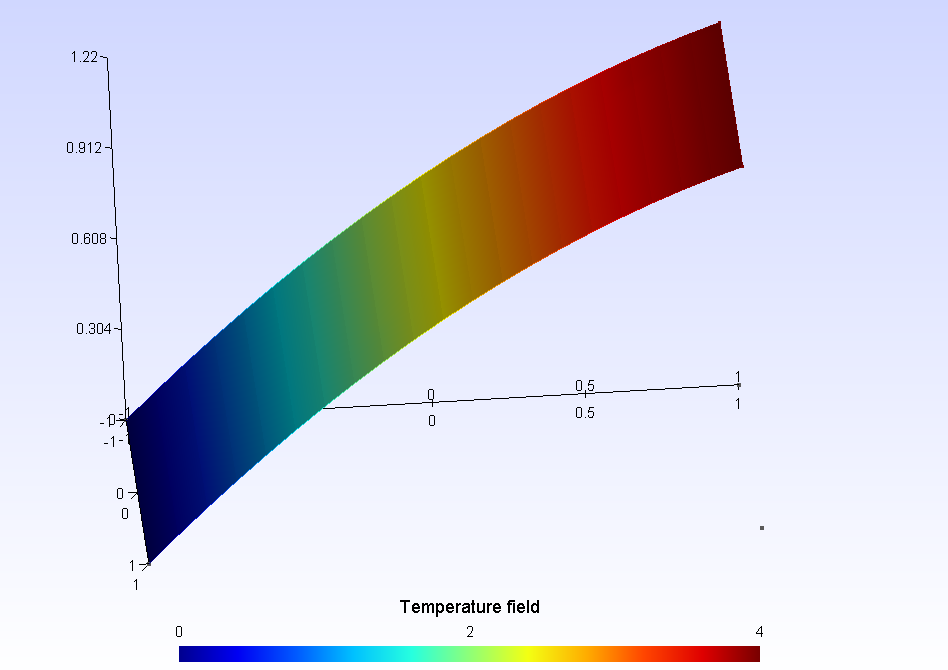
\includegraphics[width=0.75\textwidth]{FEM1}


this image is from FEM and the maximum temperature is around the same is finite difference. 

Now the solution for probelm with all side dirichlet with zero fixed temperature and hear source of one. the below image is from FEM problem, as expected we get a dome with max temperature in the middle.

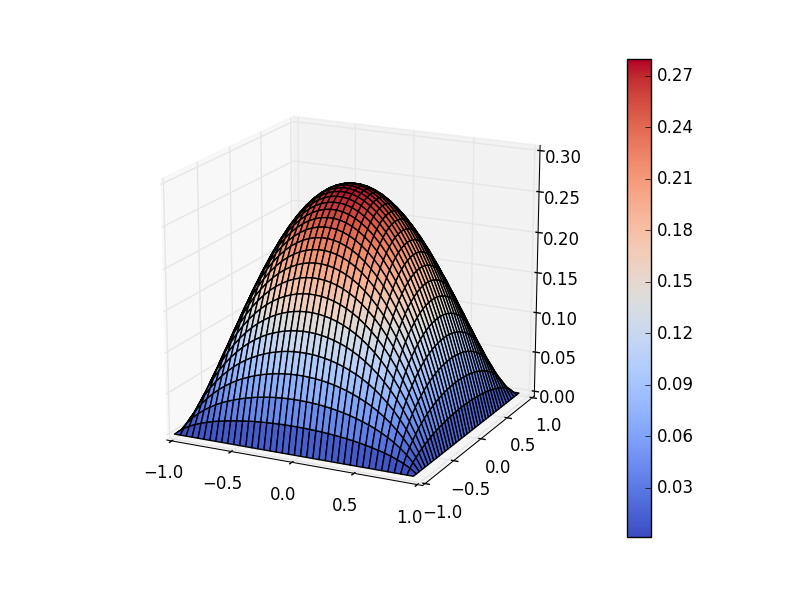
\includegraphics[width=0.5\textwidth]{FEM2}

the comparison is made with 2D finite Difference problem that we did before. below is the result of the FDM lab. as expected we get zero temperature in boundaries and maximum at the middle and results are approximately the same. 

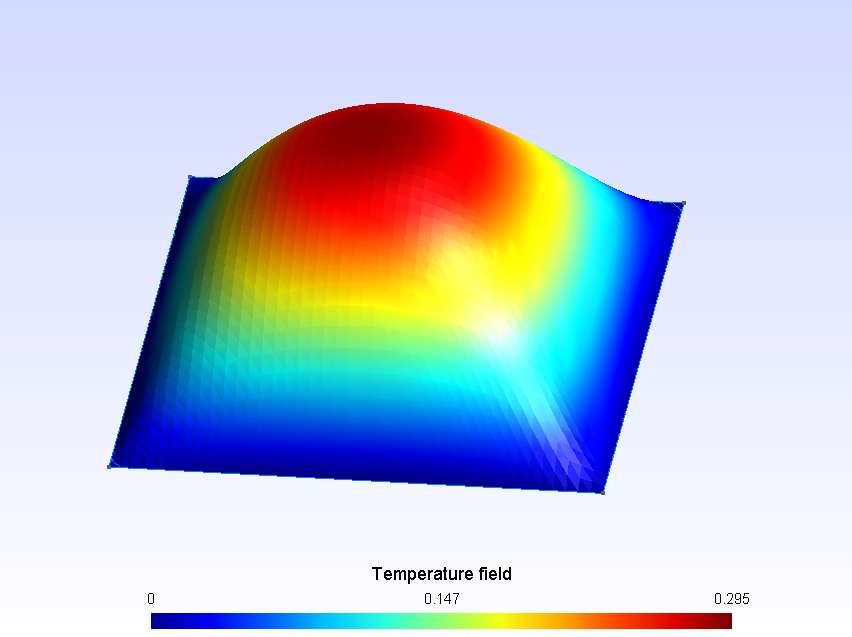
\includegraphics[width=0.75\textwidth]{FEM3}

here we use a different boundary conditions in line 101 we have applied dirichlet with 0 temperature and neumann with 1 at line 102 and dirichlet at corner 3 along with hear source 1. below is the result from FEM code.

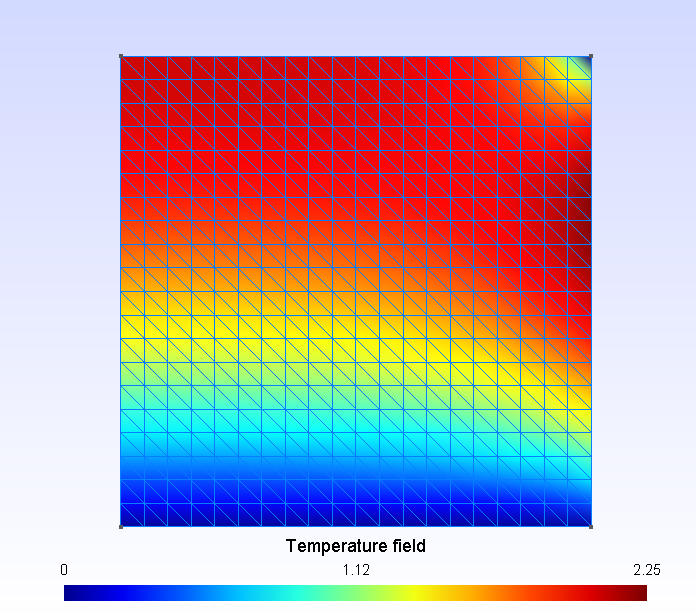
\includegraphics[width=0.75\textwidth]{FEM4}
it clearly shows that the minimum temperature are at line 101 and a point 3. 
For this boundary condition we compared with the commercial FEM software ANSYS.The results are posted in the below picture.They can clearly state that results are almost same. 
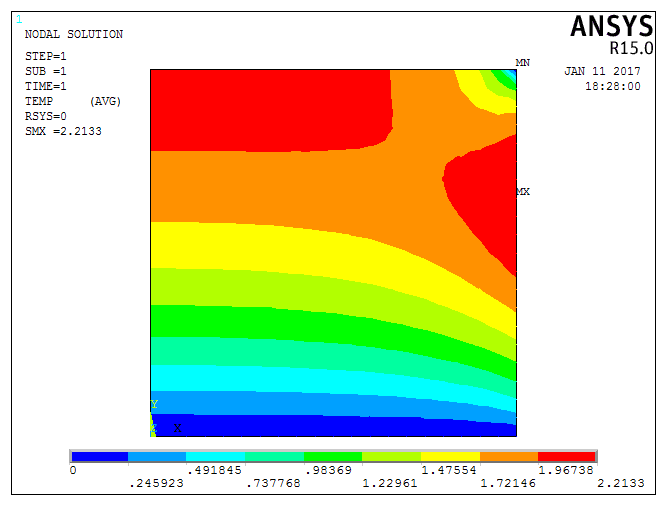
\includegraphics[width=0.75\textwidth]{FEM5}


\section{Conclusion}

The Finite Element Code is done using python and Analytical and Numerical results are compared 

 \citep{adams1995hitchhiker}

\bibliographystyle{plain}
\bibliography{references}
\end{document}
